%% Beginning of file 'SN2020jgb.tex'
%% using aastex version 6.3
\documentclass[twocolumn]{aastex631}

\newcommand\sn{SN\,2020jgb}
\newcommand\trpeak{$t_{r,\mathrm{peak}}$}
\newcommand\tfl{$t_\mathrm{fl}$}

\shorttitle{\sn}
\shortauthors{Authors et al.}
\graphicspath{{./}{figures/}}

\begin{document}

\title{\sn}

\author{Authors}
\affiliation{Center for Interdisciplinary Exploration and Research in Astrophysics (CIERA), Department of Physics and Astronomy, Northwestern University, 2145 Sheridan Road, Evanston, IL 60208, USA}

\begin{abstract}

\end{abstract}

\keywords{keywords}

\section{Introduction} \label{sec:intro}
\begin{itemize}
    \item SN 2016jhr \citep{jiang_16jhr_2017}
    \item SN 2016hnk as a double detonation \citep{jacobson-galan_16hnk_2020} or a near-Chandrasekhar mass, 91bg-like object \citep{galbany_16hnk_2019}
    \item SN 2018byg \citep{de_18byg_2019}
    \item SN 2019ofm \citep{de_Ca_rich_2020}
\end{itemize}
\section{Observations} \label{sec:obs}
\subsection{Detection and Classification}
\sn\ was first discovered by the Zwicky Transient Facility \citep[ZTF;][]{ZTF2019a,ZTF2019b} on 2020 May 03.463 UT (MJD 58972.463) with the 48-inch Samuel Oschin Telescope (P48) at Palomar Observatory. The internal designation is ZTF20aayhacx. It was detected at a magnitude of 19.86 in ZTF $g$-band, and J2000 coordinates $\alpha=17^\mathrm{h}53^\mathrm{m}12^\mathrm{s}.651$, $\delta=-00^\circ51'21''.81$. The last non-detection was on 2020 April 27.477 (MJD 58966.477; 5.99\,days before the first detection) up to a limiting magnitude of 20.7 in ZTF $r$-band.

\textbf{Classification, ...}

\subsection{Optical Photometry}
We obtained $gr$-band photometry of \sn\ with the ZTF camera. A Galactic extinction of $E(B-V)=0.404$ is reported by the maps of \citet{Schlafly2011}, for which we correct all our photometry using the extinction model proposed by \citet{Fitzpatrick1999}. We do not account for any additional host extinction due to the lack of any \ion{Na}{1} D absorption in our spectra.

\begin{figure*}
    \centering
    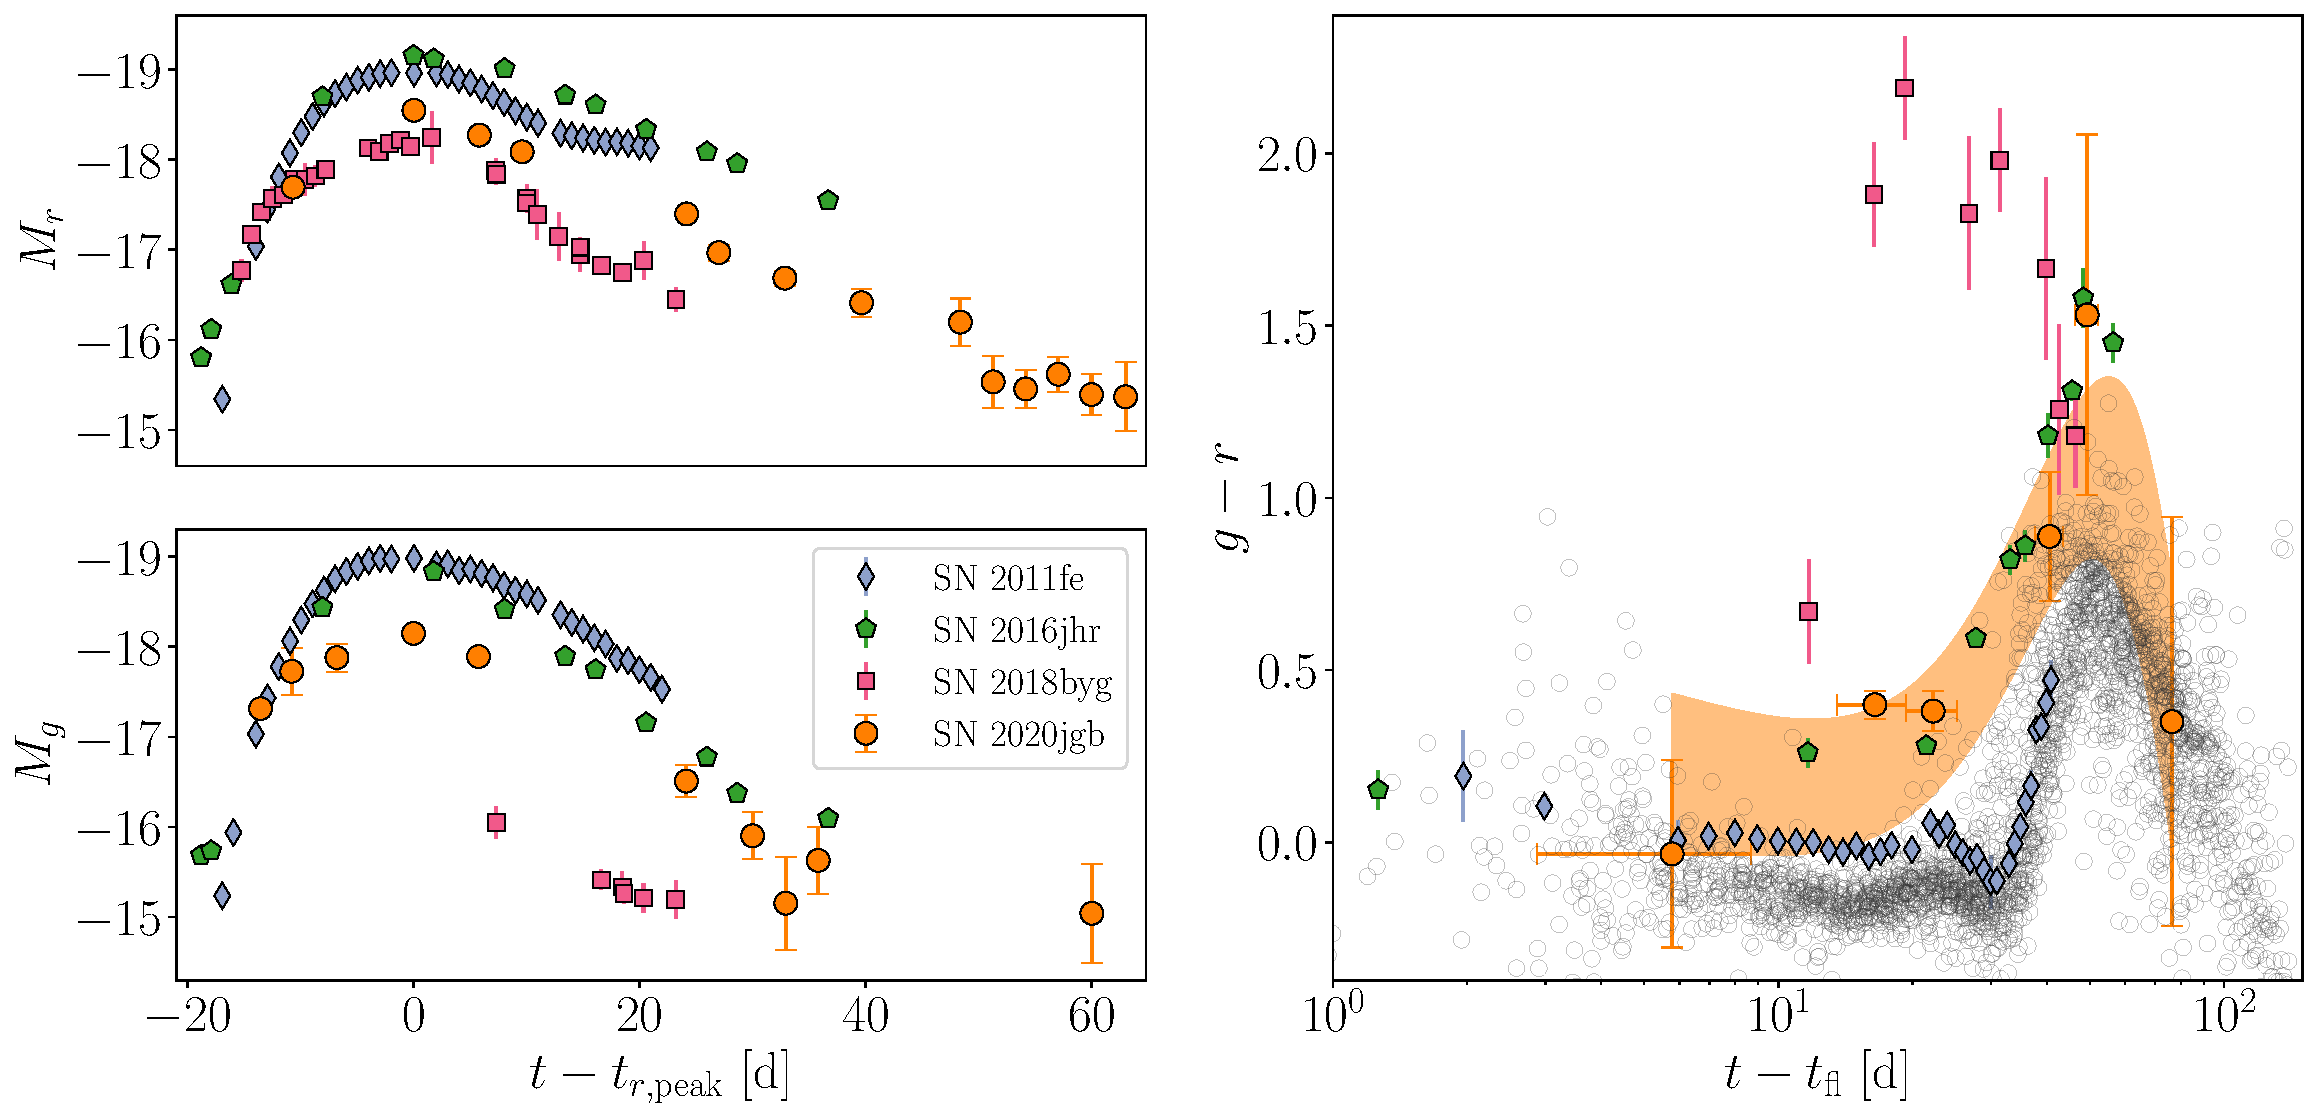
\includegraphics[width=\textwidth]{photometry.pdf}
    \label{fig:photometry}
    \caption{\textit{Left}: comparison of the multi-color ($g$ and $r$ bands) light curves of \sn\ to the normal SN Ia SN 2011fe and the He double detonation candidate SN 2018byg. \textit{Right}: comparison of $g-r$ color evolution to SN 2011fe and SN 2018byg, as well as 62 normal SNe Ia (open circles) with prompt observations within 5\,days of first light by ZTF \citep{Bulla2020}. The shaded region denotes the 1-$\sigma$ credible interval of the color of SN 2020jgb until $\sim$40\,days after the peak, estimated using Gaussian process.}
\end{figure*}

\subsection{Optical Spectroscopy}
We obtained optical spectroscopic follow-up of the object from $\approx$$-10$\,days to $\approx$$+150$\,days after the $r$-band peak, using the Spectral Energy Distribution Machine \citep[SEDM;][]{SEDM_2018} on the automated 60\,inch telescope \citep[P60;][]{P60_2006} at Palomar Observatory, the Kast Double Spectrograph \citep{miller1994kast} at the Shane 3\,m Telescope, the Andalucia Faint Object Spectrograph and Camera (ALFOSC)\footnote{\url{https://www.not.iac.es/instruments/alfosc/}} installed at the Nordic Optical Telescope (NOT), the Double Beam Spectrograph (DBSP) on the 200\,inch Hale telescope \citep[P200;][]{P200_1982}, the Low Resolution Imaging Spectrograph (LRIS) on the Keck I telescope \citep{Keck_1995}.

\begin{deluxetable}{lrcccc}
\tabletypesize{\scriptsize}
\tablewidth{0pt}
\tablecaption{Spectroscopic Observations of \sn\label{tab:spectra}}
\tablehead{
\colhead{$t_\mathrm{obs}$} &
\colhead{Phase} &
\colhead{Telescope/} &
\colhead{$R$} &
\colhead{Range} &
\colhead{Air} \\
\colhead{(MJD)} &
\colhead{(d)} &
\colhead{Instrument} &
\colhead{$(\lambda/\Delta\lambda)$} &
\colhead{(\AA)} & 
\colhead{Mass}
}
\startdata
58,976.42 &  $-$9.7 & P60/SEDM & 100 & 3770--9220 & 1.23\\
58,982.12 & $-$4.2 & NOT/ALFOSC & 360 & 4000--9620 & 1.17\\
58,990.43 &  $+$3.9 & P60/SEDM & 100 & 3770--9220 &  1.23\\
58,997.44 & $+$10.7 & P60/SEDM & 100 & 3770--9220 &  1.29\\
58,998.41 & $+$11.6 & Shane/Kast & 1000? & 3620--10720 & 1.28\\
59,008.41 & $+$21.3 & P60/SEDM & 100 & 3770--9220 & 1.28\\
59,010.40 & $+$23.3 & P200/DBSP & 700 & 3200--9500 &  1.27\\
59,023.58 & $+$36.1 & Keck I/LRIS & 1100 & 3200--10250 & 2.04\\
59,107.29 & $+$117.3 & Keck I/LRIS & 1100 & 3200--10250 & 1.31\\
59,143.26 & $+$152.2 & Keck I/LRIS & 1100 & 3200--10250 & 2.16\\
\enddata
\tablecomments{Phase is measured relative to \trpeak\ in the host galaxy rest frame. The resolution $R$ is reported for the central region of the spectrum.}
\end{deluxetable}
\begin{figure*}
    \centering
    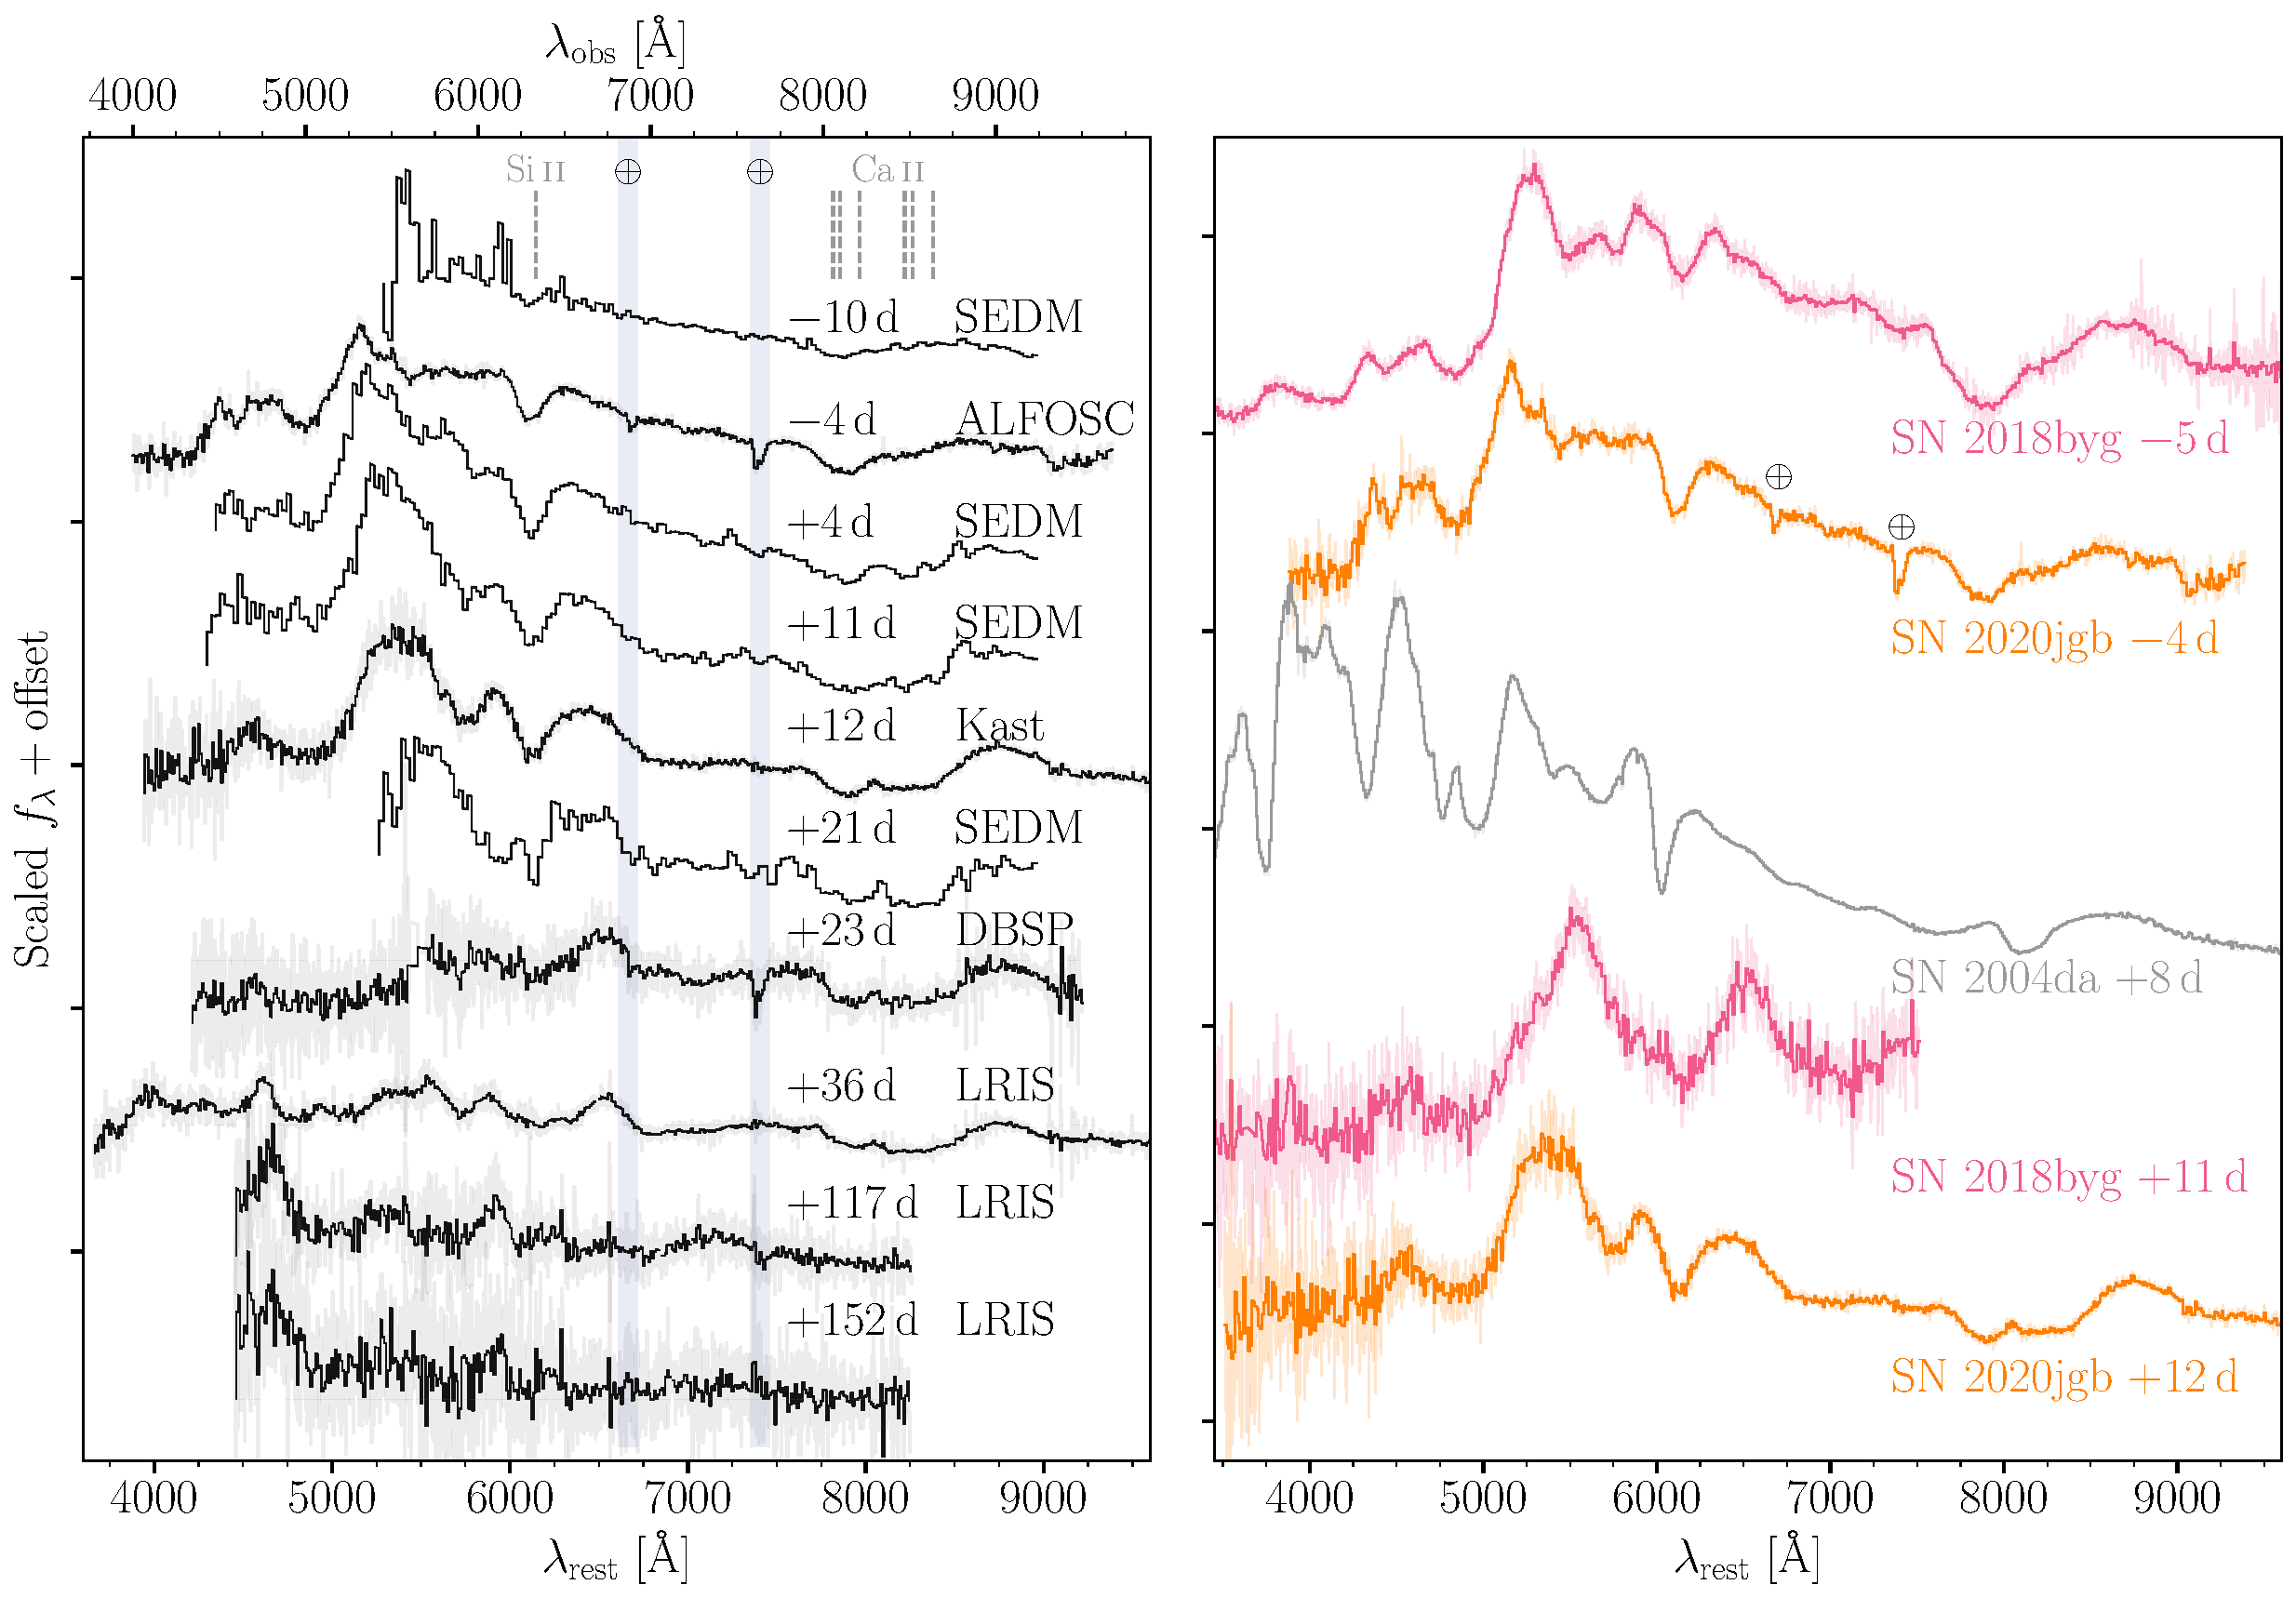
\includegraphics[width=\textwidth]{optical_spec_evolution.pdf}
    \caption{Optical spectroscopic sequence of \sn. Rest frame phases (days) relative to the $r$-band peak and instruments used are posted next to each spectrum. The black curves are binned spectra with a bin size of 10\,\r{A}, except for the SEDm spectra, whose resolution is lower. The 1-$\sigma$ uncertainties of raw spectra are shown in grey. Only regions with SNR $>3$ after binning are plotted.} %The \ion{Si}{2} and \ion{Ca}{2} IRT absorption lines are indicated by the vertical dashed lines. The telluric lines are denoted by the earth symbol, ``$\earth$''.
    \label{fig:spec_evo}
\end{figure*}

\subsection{Near-infrared (NIR) Spectroscopy}
We obtained one NIR (0.8-2.5\,\micron) spectrum of the transient using the Gemini near-infrared spectrometer \citep[GNIRS;][]{GNIRS1998} on the Gemini North telescope on 2020 June 9 ($\approx$22\,days after $r$-band peak), for an integration time of 2400 s. The spectra were reduced with the \texttt{PypeIt} Python package \citep{pypeit:joss_pub,pypeit:zenodo}.

\begin{figure*}
    \centering
    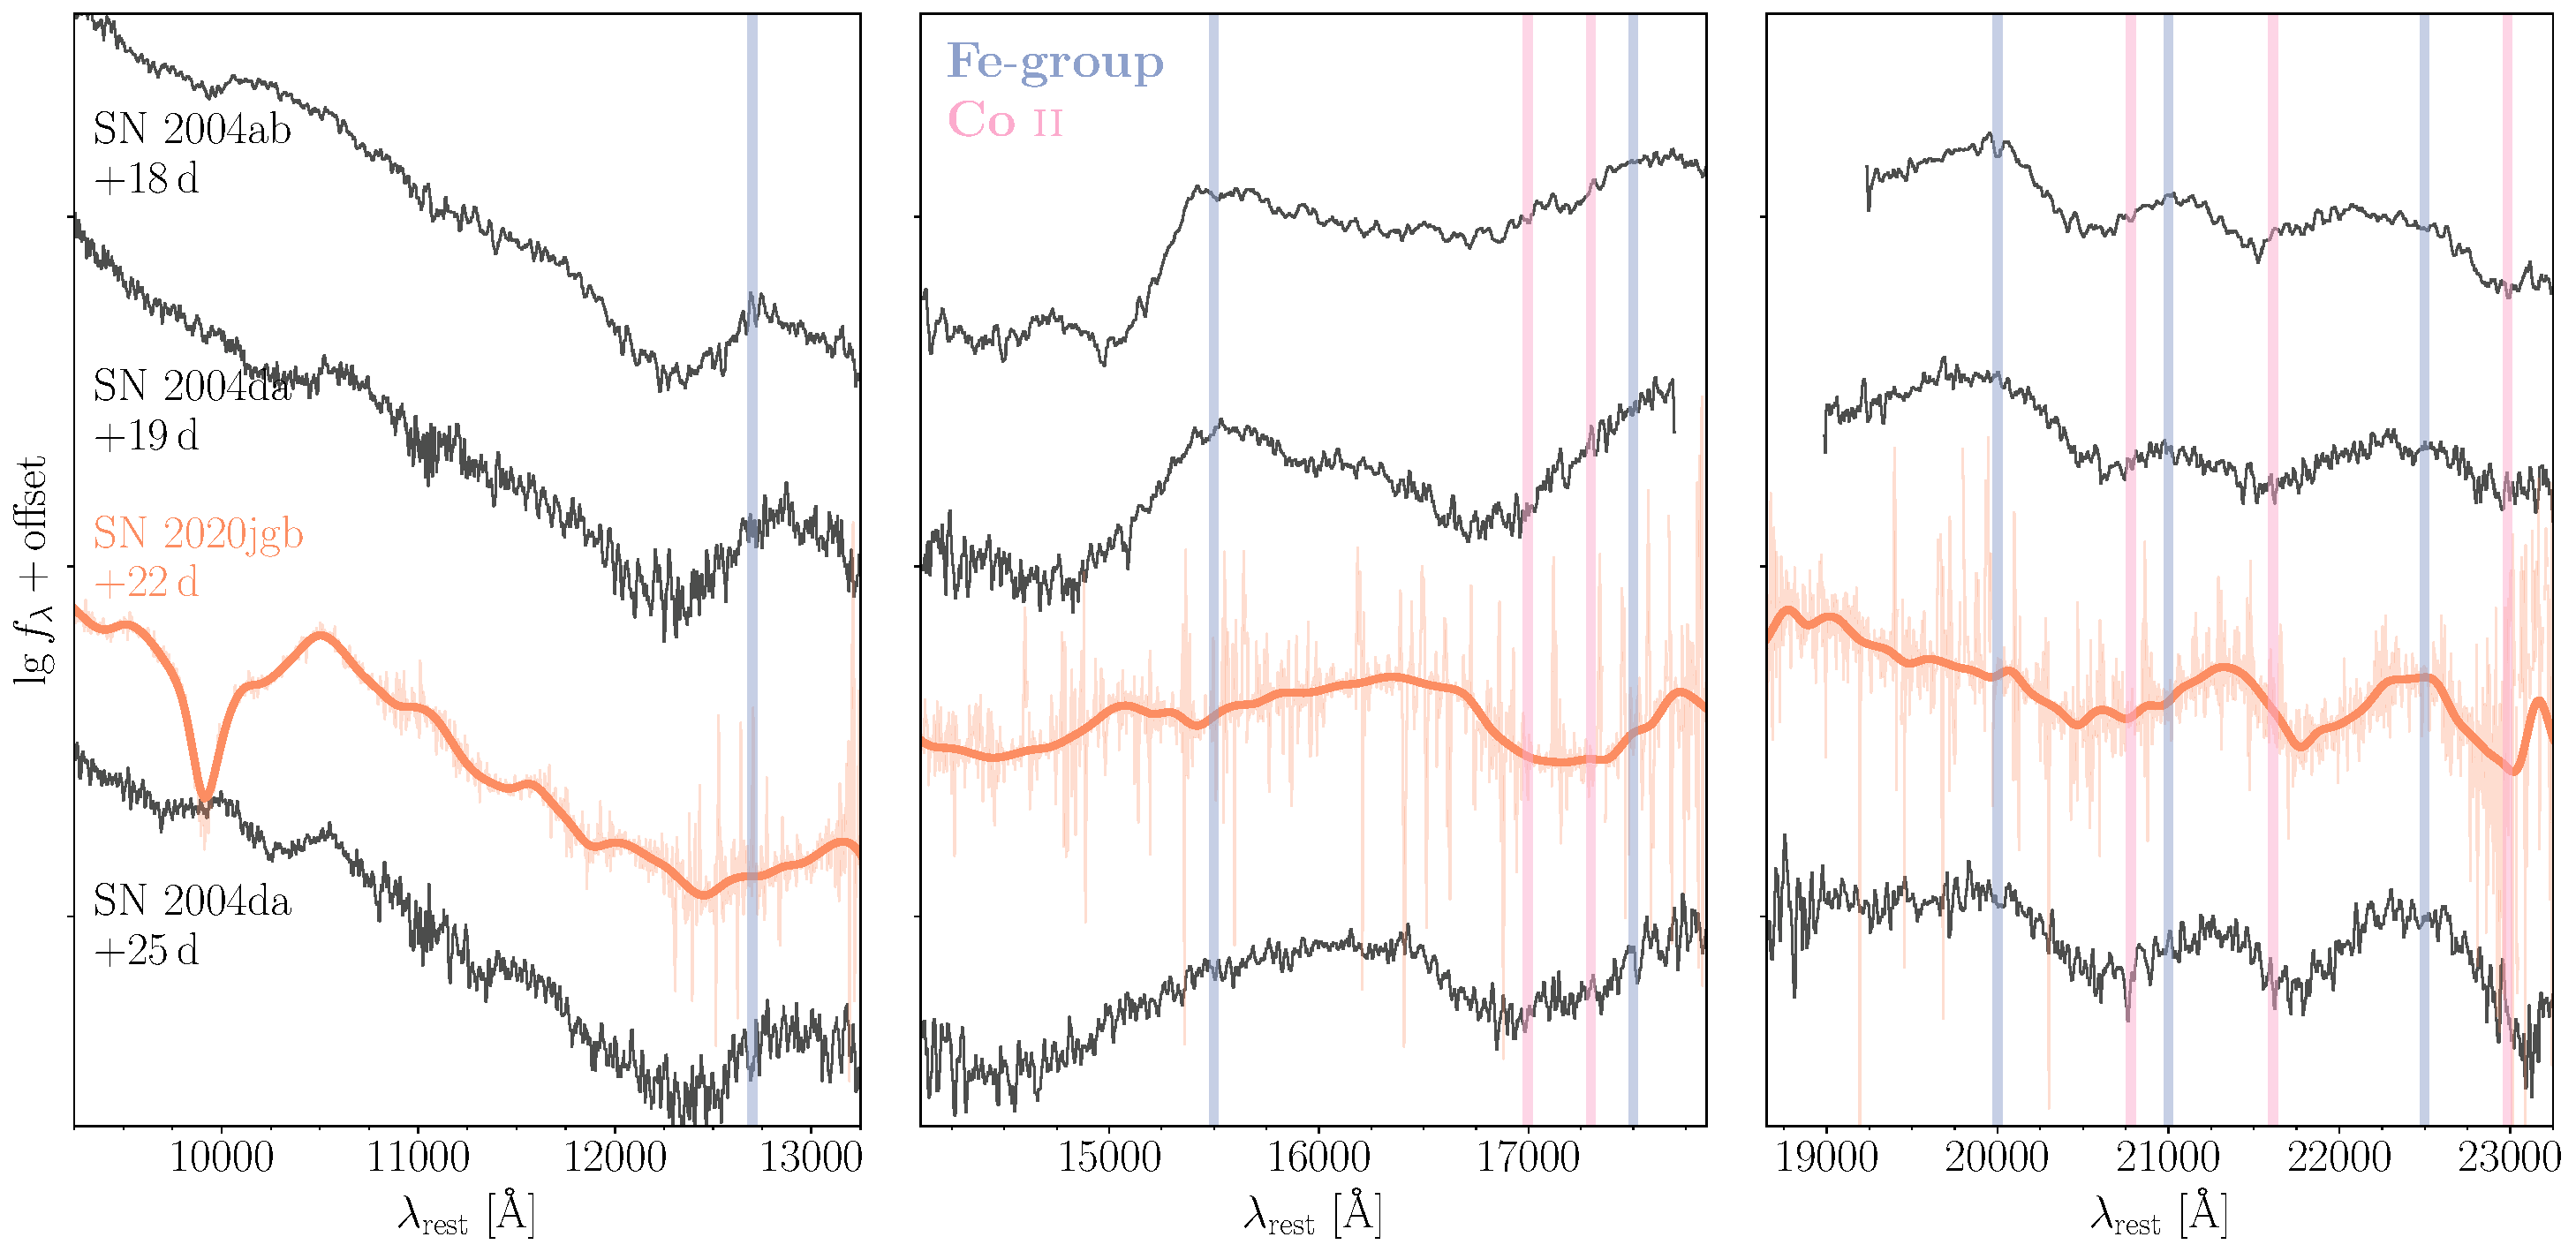
\includegraphics[width=\textwidth]{NIR_spec.pdf}
    \caption{The NIR spectra of \sn\ and two SNe Ia with normal maximum luminosity \citep[SN 2004ab and SN 2004da,][]{Marion2009_NIR}, taken about three weeks after the peak. For each spectrum, the continuum at $\gtrsim1.2$\,\micron\  is significantly reshaped by the Fe-group blanketing (emission features, blue vertical lines) and \ion{Co}{2} absorption (pink vertical lines).}
    \label{fig:NIR_spec}
\end{figure*}

\section{Analysis} \label{sec:analysis}
\subsection{Photometric Properties}
\sn\ exhibited a fainter light curve than normal SNe Ia. In Figure~\ref{fig:photometry}, we compare the photometric properties of \sn\ with the canonical SN Ia SN2011fe \citep{Nugent_11fe_2011} and two He-shell double detonation candidates, SN 2016jhr and SN 2018byg. The photometric data are taken from the Open Supernova Catalog \citep{Guillochon_2017}.

The first detection was made on MJD=58972.46 in ZTF $g$-band. At a similar phase relative to the peak light, the luminosity was similar to the canonical object SN 2011fe and also the two double detonation candidates. But since then the light curve showed a slower rise than both SN 2011fe and SN 2016jhr, yet still faster than SN 2018byg. Near peak, the double detonation sample is heterogeneous in luminosity. The decline rate in $g$-band of \sn\ is similar as normal-luminosity SNe Ia, hence much slower than usual sub-luminous objects. SN 2018byg also seemed to exhibit an unusually slow decay in $g$-band, though the $g$-band peak was not covered.

In the right panel of Figure~\ref{fig:photometry}, we also compare the color evolution (ZTF $g-r$) of these objects as measured from their first light $t_\mathrm{fl}$, accompanied by 62 normal SNe Ia (open circles) observed within 5 days of $t_\mathrm{fl}$ by ZTF \citep[from][]{Bulla2020}. For \sn\, the early rise of the light curve was not well sampled, so we take the midpoint of the first detection and the last none-detection as an approximation of the explosion time, with the uncertainty ($\approx$3\,days) being half of the offset between these two epochs. We also evaluate the 1-$\sigma$ uncertainty of the $g-r$ color (the shaded region) in \sn\ by fitting the light curve in each band with Gaussian process. All three double detonation candidates are undoubtedly redder than normal SNe Ia. At peak light, \sn\ was not as red as the extreme case, SN 2018byg ($g-r\approx2.2$), while exhibited a similar color evolution as SN 2016jhr ($g-r\approx0.5$). Nonetheless, the colors eventually converged at $\sim$50\,days after the first light, suggesting that the unusually red colors were not due to uncorrected dust extinction \citep{de_18byg_2019}.

\subsection{Optical Spectral properties}
In Figure~\ref{fig:spec_evo}, we show the optical spectral sequence of \sn, and compare its spectra with some other SNe Ia near peak luminosity. The earliest spectrum was obtained by SEDM $\approx$10\,days before the $r$-band peak. The signal-to-noise ratio (SNR) is sufficiently high only at $\gtrsim$5500\,\r{A}, where the continuum is almost featureless with some marginal detection of the \ion{Si}{2} features at $\approx$6100\,\r{A}, the trademark of SNe Ia. In subsequent spectra the \ion{Si}{2} features become much more prominent and linger on until at least $\sim$10\,days after the peak light. We fit the \ion{Si}{2} feature with a Gaussian profile to get an expansion velocity of $\approx$11,500\,km/s near peak light. 

Also in the earliest spectrum, the wide absorption features by \ion{Ca}{2} infrared triplet (\ion{Ca}{2} IRT) have been visible at about 7800-8200\,\r{A}. We fit the absorption features assuming each line in the triplet can be approximated by the same Gaussian profile (i.e., same amplitude and dispersion), and obtained a best-fit expansion velocity $\gtrsim$26,000\,km/s. Such high-velocity features (HVFs) remain visible for over 40\,days. The photospheric velocity features (PVFs) at about 8200-8600\,\r{A} is not visible until in our second spectrum $\approx$4\,days before peak light. Since then we fit the broad absorption features with two different velocity components simultaneously. The velocity of HVFs slightly declines but stays above $\approx$24,000\,km/s, and the velocity of PVFs declines from $\approx$11,000\,km/s to $\approx$9,000\,km/s. As in normal SNe Ia, the relative strength between HVFs and PVFs decreases with time.

\sn\ highly resembles other double detonation candidates (e.g., SN 2018byg and SN 2016hnk) in (i) the strong continuous absorption blueward of $\approx$5000\,\r{A}, which is believed to be the line blanketing of Fe-group elements synthesized in the helium shell burning, and (ii) the wide absorption feature of \ion{Ca}{2} IRT, with the HVFs being prominent. Such high spectral similarity in makes \sn\ another promising candidate for He-shell double detonation SN.

In \S\ref{sec:NIR_spec} we will discuss the NIR spectra of \sn, where \sn\ also resembles the normal-luminosity SN Ia, SN 2004da (see Figure~\ref{fig:NIR_spec}). Hence we also exhibit one of the optical spectra of SN 2004da in Figure~\ref{fig:spec_evo}, which is typical for a normal SN Ia and does not show any suppress of flux in $g$-band, as the sub-luminous double detonation objects do. It also lacks the HVFs of \ion{Ca}{2} IRT.

\subsection{NIR Spectral properties}
\label{sec:NIR_spec}
In Figure~\ref{fig:NIR_spec}, the NIR spectrum is presented along with three spectra in the sample of \cite{Marion2009_NIR} at similar phases. \sn\ shows a strong absorption feature at $\approx$0.99\,\micron, which is not seen in normal SNe Ia. This feature was still significant two weeks later, as detected by LRIS on Keck (see Figure~\ref{fig:hvf_comp}), though it was only partially covered due to the limitation of bandwidth. In general, \sn\ highly resembles normal SNe Ia in NIR band. The shape of the continuum redwards to $\approx$1.2\,\micron\ is significantly altered by line-blanketing of Fe-group elements synthesized in the SN interior, as opposed to the Fe-group elements in the outermost region as ashes of shell helium burning. Just like normal SNe Ia, \sn\ also show enhancement of flux at about 1.3, 1.55, 2.0, 2.1, and 2.25\,\micron, accompanied by several \ion{Co}{2} absorption lines. It is especially similar to SN 2004da at +25\,days after maximum as the steep increase in flux at $\approx$1.55\,\micron, known as the \textit H-band break, has become less prominent. %For many other SNe Ia, however, the \textit H-band break can last till much later stages \citep{Marion2009_NIR}.

What is not seen in usual SNe Ia is the wide, deep absorption at $\approx$0.99\,\micron\ (hereafter the 1\,\micron\ feature), indicating its peculiarity. According to \citet{Marion2009_NIR}, normal SNe Ia are nearly featureless in spectra around 1\,\micron\ a few weeks past the week. There are several elements that may be associated with this feature. None of these identifications is fully satisfying, and usually other strong lines of the same elements are missing in the spectra. The nature of the 1\,\micron\ feature remains uncertain. Chances are that this absorption is a mixture of multiple weaker lines.

The most attractive possibility is the strong \ion{He}{1} line at 1.0830\,\micron, as has predicted in sub-Chandrasekhar-mass He-shell double detonation models when considerable amount of helium in the shell is left unburnt \citep{Boyle2017_Helium}. Figure~\ref{fig:hvf_comp} shows that the 1\,\micron\ feature, if associated with \ion{He}{1} $\lambda$1.0830\,\micron, has a high velocity ($\approx$26,000\,km/s), yet similar as the HVF of \ion{Ca}{2} IRT ($\approx$24,000\,km/s). The expansion velocity in the ejecta is roughly linearly proportional to the radius, so such a high velocity indicates that both the \ion{Ca}{2} IRT and the tentative \ion{He}{1} absorption line form far outside the normal photosphere, which has a velocity of only $\approx$10,000\,km/s. In the sense, the He-shell double detonation scenario, in which the unburnt helium locates at the outermost ejecta, is indeed supported.
\begin{figure}
    \centering
    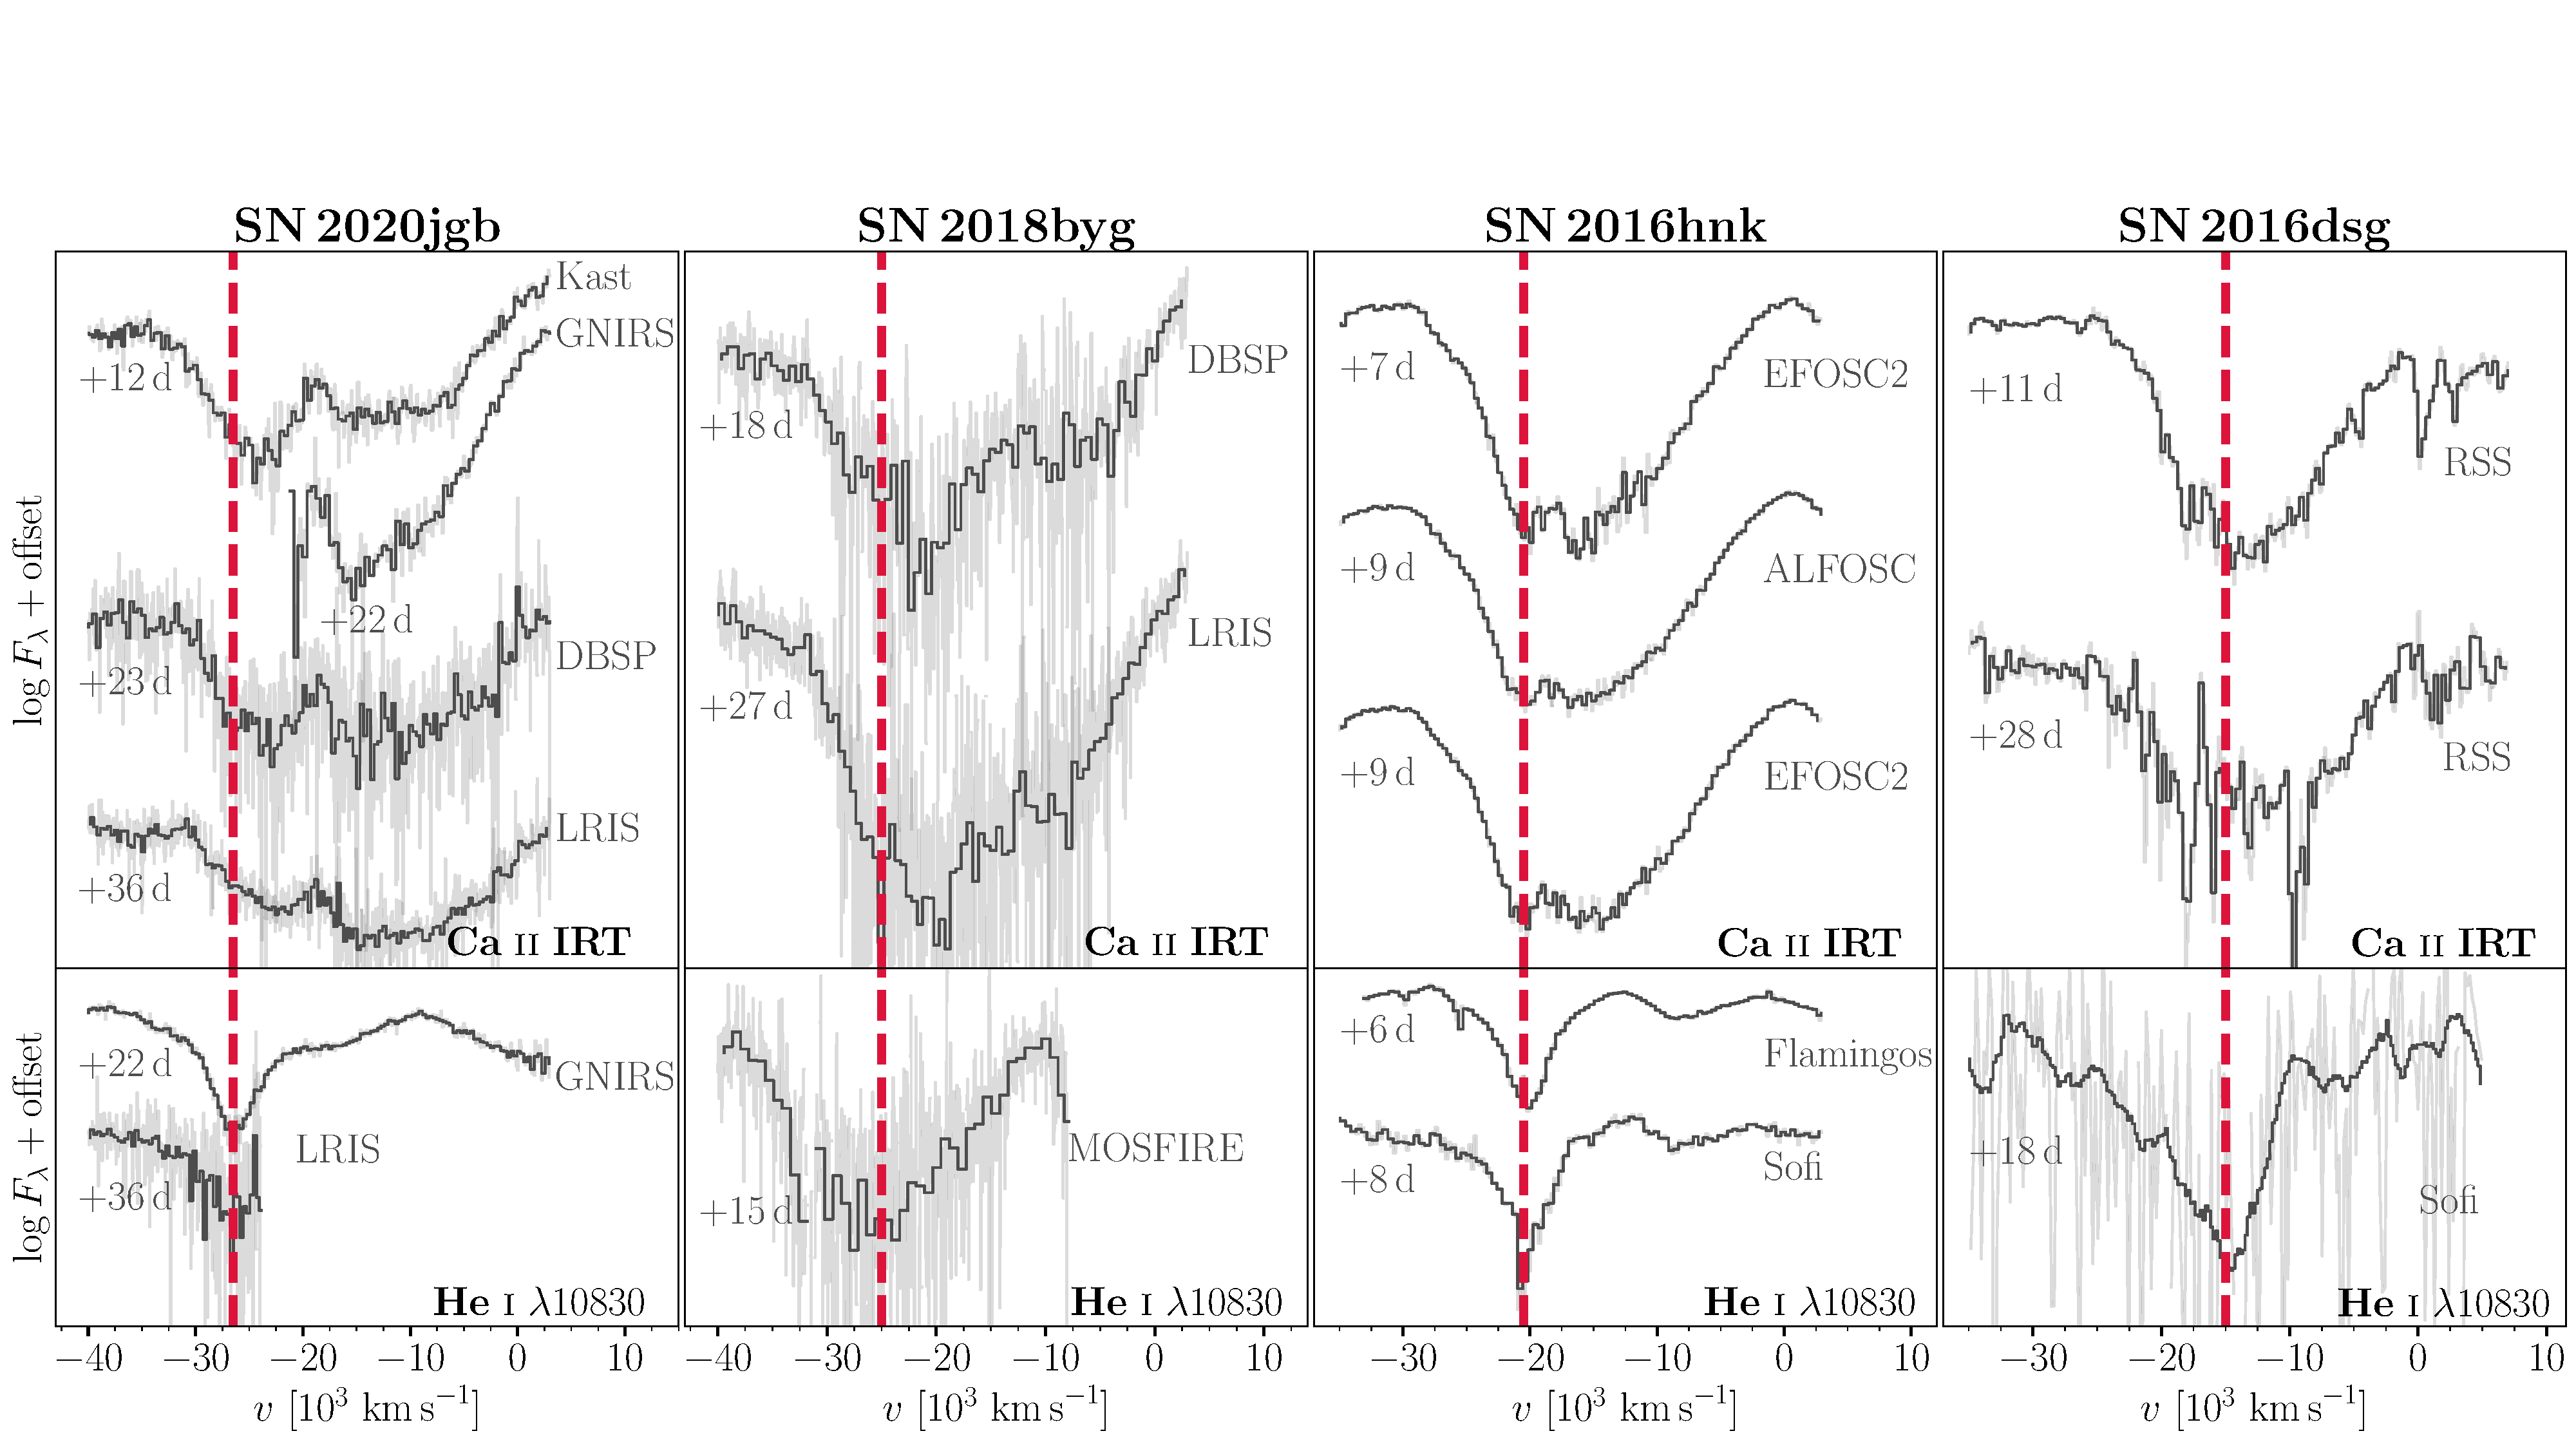
\includegraphics[width=\linewidth]{CaII_HeI_hvf.pdf}
    \caption{Spectra in the velocity space, comparing the high-velocity component of \ion{Ca}{2} IRT and the absorption feature at $\approx$0.99\,\micron\ assuming it is associated with \ion{He}{1} at 1.0830\,\micron.}
    \label{fig:hvf_comp}
\end{figure}

Still, this helium detection remains skeptical, since other \ion{He}{1} are not unambiguously detected, such as the \ion{He}{1} $\lambda$2.0581\,\micron. Considering a line velocity of $\approx$26,000\,km/s and a host galaxy redshift of 0.0307, this line will be blueshifted to $\approx$1.95\,\micron\ in the observer frame, so will be strongly blended by the strong telluric lines within 1.8-2.0\,\micron. After telluric correction, the signal to noise ratio reaches $\sim$5, with which we still cannot see any significant absorption feature. An upper limit of the equivalent width is determined to be $<2\%$ of the 1.0830\,\micron\ line, while theoretically, the 2.0581\,\micron\ line is supposed to be only a factor of 6-12 weaker, depending on temperature \citep{Marion2009_NIR}. Another fact is that the 1\,\micron\ feature is as strong as the \ion{He}{1} $\lambda$1.0830\,\micron\ in many helium-rich core-collapse supernovae, say, Type Ib supernovae, in which the \ion{He}{1} $\lambda$2.0581\,\micron\ is weaker than the 1.0830\,\micron\ line yet still prominent \citep{CSP_Ibc_2022}. If the 1\,\micron\ feature is associated with \ion{He}{1}, it would be very unusual if the 2\,\micron\ feature is not seen at all, even if somehow blended by the telluric lines.

Other possibilities include the \ion{Mg}{2} $\lambda$1.0927\,\micron, the \ion{C}{1} $\lambda$1.0693\,\micron, and the \ion{Fe}{2} $\lambda$1.0500\,\micron\ \& $\lambda$1.0863\,\micron. The \ion{Mg}{2} $\lambda$1.0927\,\micron\ line is prevalent in the NIR spectra of SNe Ia, but usually disappears within a week after the peak luminosity \citep{Marion2009_NIR}, while the 1\,\micron\ feature was still visible over a month after the peak in the Keck LRIS spectrum. The required radial velocity is $\approx$30,000\,km/s, $\approx$20\% faster than the HVF of \ion{Ca}{2} IRT at the same phase. While such a high velocity for \ion{Mg}{2} has never been seen in other SNe Ia, since high-velocity intermediate-mass elements like magnesium and calcium can be synthesized by the detonation of helium shell \citep{Shen_DD_2014}, the \ion{Mg}{2} origin of the 1\,\micron\ feature cannot be strictly ruled out. But if we attribute this 1\,\micron\ feature to high-velocity \ion{Mg}{2}, we would expect an even stronger $\lambda$0.9227\,\micron\ line to be blueshifted to the red edge of the \ion{Ca}{2} IRT, which is not detected. Given the strength of the 1\,\micron\ feature, the 0.9227\,\micron\ line should not be completely obscured by the \ion{Ca}{2} IRT features. 

The \ion{C}{1} $\lambda$1.0693\,\micron\ line from the unburnt carbon is much less frequently seen than the \ion{Mg}{2} $\lambda$1.0927\,\micron. \citet{hsiao_CSP_2019} presented a sample of five SNe Ia with \ion{C}{1} detections, showing the \ion{C}{1} feature is strongest for those fainter, fast-declining objects. However, in their sample, the \ion{C}{1} feature is a pre-maximum feature which fades away as the luminosity peaks, so the discrepancy in phase is large. The required expansion velocity $\approx$22,000\,km/s, which is overwhelmingly faster than the estimated carbon velocity for the sample in \citet{hsiao_CSP_2019} ($\sim$10,000-12,000\,km/s), but still consistent with the HVF of \ion{Ca}{2} IRT. Nonetheless, no significant carbon absorption is detected in the optical band.

The \ion{Fe}{2} features in SNe Ia usually start to develop roughly three weeks after the peak, which is about the same phase as we obtained our GNIRS spectrum. Two \ion{Fe}{2} lines, $\lambda$0.9998\,\micron\ and $\lambda$1.0500\,\micron, are actually visible on the blue/red wings of the 1\,\micron\ feature. The \ion{Fe}{2} $\lambda$1.0863\,\micron\ line is not yet seen in the GNIRS spectrum. They correspond to an expansion velocity of $\approx$8,000\,km/s, which is consistent with the PVF of the \ion{Ca}{2} IRT at the same epoch. They also match the same two lines for normal SNe Ia \citep{Marion2009_NIR}, making the identification more reliable. Obviously, these two \ion{Fe}{2} features are wider and shallower than the strong feature between them. We fit the 1\,\micron\ feature with three Gaussian profiles. Two of them are set to be the blueshifted \ion{Fe}{2} $\lambda$0.9998\,\micron\ and $\lambda$1.0500\,\micron, and the other is an uncorrelated Gaussian profile which mainly describes the absorption in the center. We find that the shallower and wider \ion{Fe}{2} lines only make up $\sim$40\% of the total equivalent width, and the rest $\sim$60\% comes from the central feature, which cannot be accounted for by any \ion{Fe}{2} feature at the same velocity. Given the similarity of the Fe-group line blanketing between the GNIRS spectrum with the spectrum of SN 2004da at +25\,days, the distribution of Fe-group elements inside each supernova ejecta should be somehow similar as normal SNe Ia, so the central region of the 1\,\micron\ feature is not likely to be associated with \ion{Fe}{2} either.

While the nature of the 1\,\micron\ feature remains uncertain, other He-shell double detonation candidates also seem to show similar complexity in this region. In the currently small sample of five candidates, two objects (SN 2016jhr and SN 2019ofm) do not have any available NIR spectra, while the other three (at quite different phases though) all exhibit strong absorption features near 1\,\micron, as shown in Figure~\ref{fig:NIR_comp}. The 1\,\micron\ feature for SN 2016hnk lies at a longer wavelength than \sn, which corresponds to a lower expansion velocity, assuming they all have the same origin. The line velocity assuming a \ion{He}{1} $\lambda$1.0830\,\micron\ origin is $\approx$21,000\,km/s, which, just like \sn, is about the same as the HVF of the \ion{Ca}{2} IRT in the optical spectra. The PVF of the \ion{Ca}{2} IRT ($\approx$10,000\,km/s) is not significantly slower than that in \sn. For SN 2018byg, the velocity of the 1\,\micron\ feature with respective to the \ion{He}{1} $\lambda$1.0830\,\micron\ is still consistent with the HVF of \ion{Ca}{2} IRT. But given its exotic width and lower signal-to-noise ratio, the exact line velocity is hard to determine. It is highly likely to be a mixture of several different lines. 

Unfortunately, the NIR spectra for both SN 2016hnk and SN 2018byg do not cover the 2\,\micron\ region, thus it is not possible to identify the presence of helium decisively. But if the 1\,\micron\ feature of the these objects are of the same origin, they are more likely to be correlated with the high velocity ejecta lying in the outmost region in the supernovae, because at least for \sn\ and SN 2016hnk, the difference in their photospheric velocities cannot explain their discrepancy in the line velocities of the 1\,\micron\ feature. Then helium is still a promising candidate to cause strong absorption near 1\,\micron\ for these sub-luminous He-shell double detonation SNe Ia. 

Alternatively, since the NIR spectra for the three objects were all obtained at different epochs, each 1\,\micron\ feature can be of completely unrelated origin. This is to be confirmed in a more complete NIR spectral sequence in future He-shell double detonation SNe Ia. Even so, the seemingly ubiquitous 1\,\micron\ feature in various phases is possibly a distinctive attribute against normal SNe Ia.

\begin{figure}
    \centering
    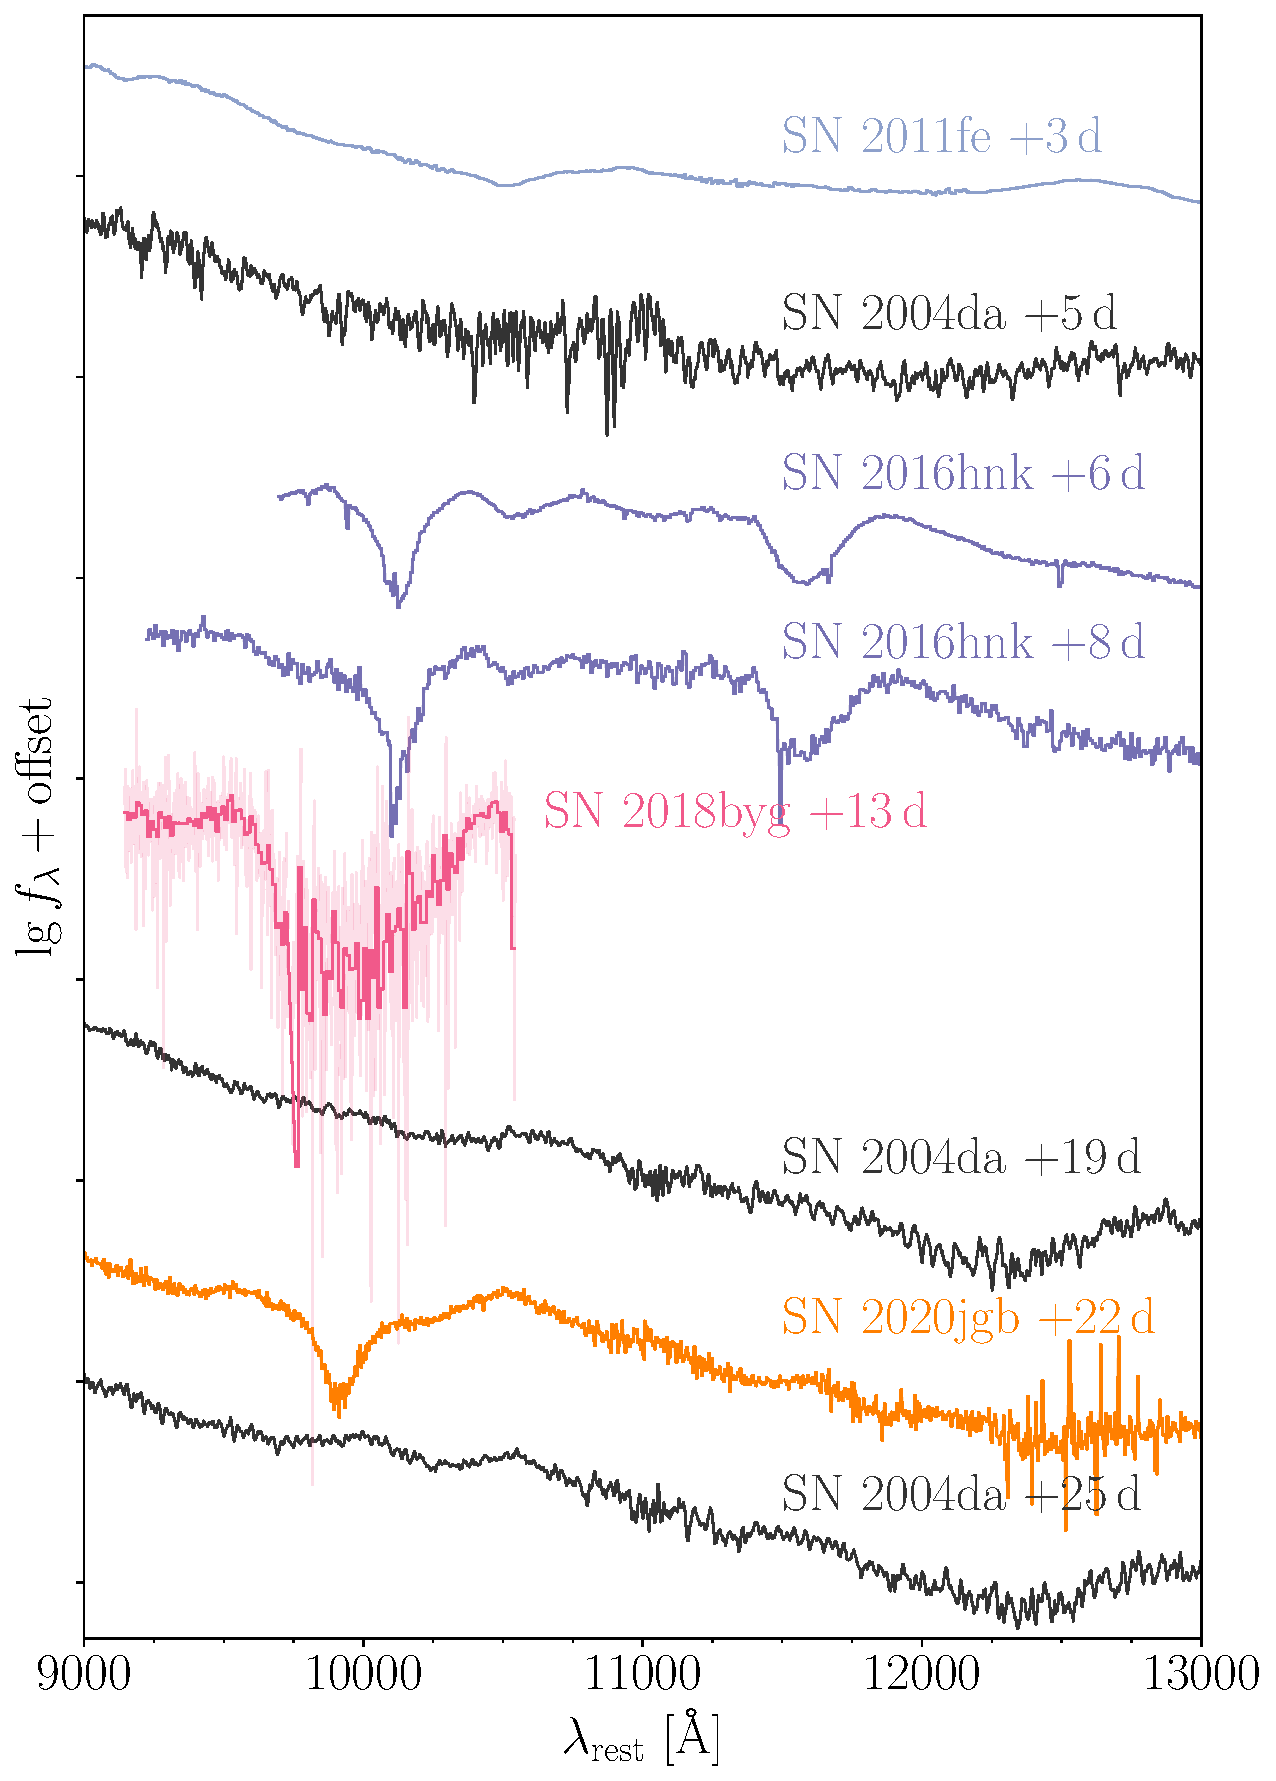
\includegraphics[width=\linewidth]{NIR_spec_comp.pdf}
    \caption{The NIR spectra (9,000 to 13,000 \AA) of a few normal SNe Ia (SN 2011fe and SN 2004da) and three He-shell double detonation candidates, which are all subluminous SNe Ia (SN 2016hnk, SN 2018byg, and this source, \sn). Spectra for SN 2004da were obtained from \citet{Marion2009_NIR}, and other spectroscopic data were obtained from the WISEReP repository \citep{wiserep_2012}.}
    \label{fig:NIR_comp}
\end{figure}

\section{Host Galaxy} \label{sec:host}
\begin{figure}
    \centering
    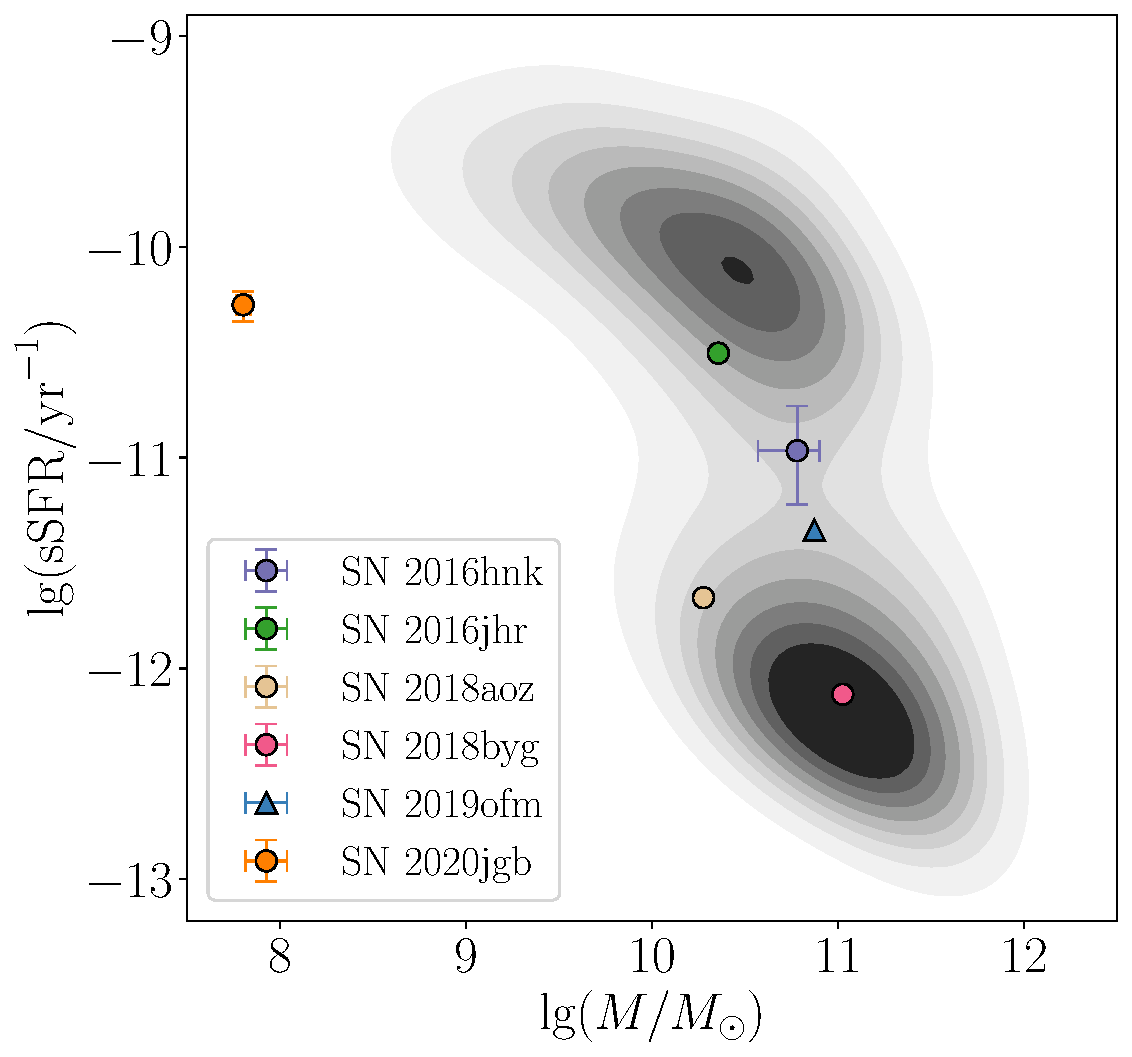
\includegraphics[width=\linewidth]{host.pdf}
    \label{fig:host}
    \caption{The specific star formation rate (sSFR) and the galactic mass for the host galaxies of He-shell double detonation candidates. The data for the host of SN 2016hnk are taken from \citet{galbany_16hnk_2019}, and for hosts we apply the galaxy parameters from the SDSS MPA-JHU DR8 catalog \citep{Kauffmann_SDSS_2003,Brinchmann_SDSS_2004}.}
\end{figure}

\section{Model Comparisons} \label{sec:model}

\section{Discussion and Conclusion} \label{sec:discussion}

\bibliography{SN2020jgb}{}
\bibliographystyle{aasjournal}

%% This command is needed to show the entire author+affiliation list when
%% the collaboration and author truncation commands are used.  It has to
%% go at the end of the manuscript.
%\allauthors

%% Include this line if you are using the \added, \replaced, \deleted
%% commands to see a summary list of all changes at the end of the article.
%\listofchanges

\end{document}

% End of file `sample631.tex'.
